% Figure 1
\ffigbox[\FBwidth]{
\caption{\centering Graphe \(G_1\) dé départ}\label{Fig:td5ex2c1}
}{
    \fbox{
        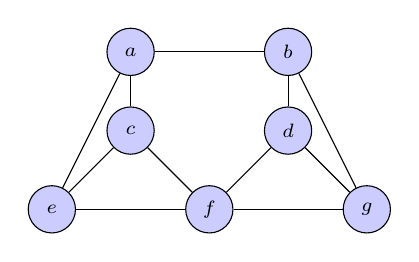
\begin{tikzpicture}[scale=1,
            main node/.style={circle, draw, fill=blue!20, inner sep=1pt, font=\scriptsize, minimum size=6mm}]
            \node[main node] (a) at (0, 0) {\(a\)};
            \node[main node] (b) at (2, 0) {\(b\)};
            \node[main node] (c) at (0, -1) {\(c\)};
            \node[main node] (d) at (2, -1) {\(d\)};
            \node[main node] (e) at (-1, -2) {\(e\)};
            \node[main node] (f) at (1, -2) {\(f\)};
            \node[main node] (g) at (3, -2) {\(g\)};
            
            \draw (a) -- (b);
            \draw (a) -- (c);
            \draw (a) -- (e);

            \draw (b) -- (d);
            \draw (b) -- (g);

            \draw (c) -- (e);
            \draw (c) -- (f);

            \draw (d) -- (f);
            \draw (d) -- (g);

            \draw (e) -- (f);

            \draw (f) -- (g);
        \end{tikzpicture}
    }
}